\documentclass[]{article}

\usepackage{graphicx}
\usepackage[margin=1in,letterpaper]{geometry}
\usepackage[final]{hyperref}
\usepackage{listings}
\usepackage{appendix}
\usepackage{amsmath}
\usepackage{float}


%opening
\title{CompArch HW2}
\author{David Abrahams}

\begin{document}

\maketitle

\section{The binary adder}

The binary adder takes in three bits: $A$, $B$, and the carry-over from the previous addition.

\subsection{The sum bit}

It outputs a $Sum$ bit, and a carry-over bit. $Sum=1$ if an odd number of the inputs are true. An odd number of the inputs are true if either of these conditions are met:
	
\begin{itemize}
			
	\item Both or neither of $A$ and $B$ are $1$, and $CarryIn$ is $1$
	\item One of $A$ and $B$ is $1$, and $CarryIn$ is $0$
	      		      
\end{itemize}
	
We can express this in boolean logic:
	
\begin{align}
	Sum & = \left(A \oplus B\right) \oplus CarryIn 
\end{align}
	
\subsection{The CarryOut bit}

$CarryOut=1$ if an two or more of the inputs are true. One of these conditions must be met met:
	
		
\begin{itemize}
			
	\item $A$ and $B$ are $1$.
	\item One of $A$ and $B$ is $1$, and $CarryIn$ is $1$
	           
\end{itemize}
	
In boolean logic:
	
\begin{align}
	CarryOut & = \left(A \& B\right) || \left(\left(A \oplus B\right) \& CarryIn\right) 
\end{align}
	
See Figure~\ref{adder} for the implementation in a circuit.
	
\begin{figure}[H]
	\label{adder}
	\centering
	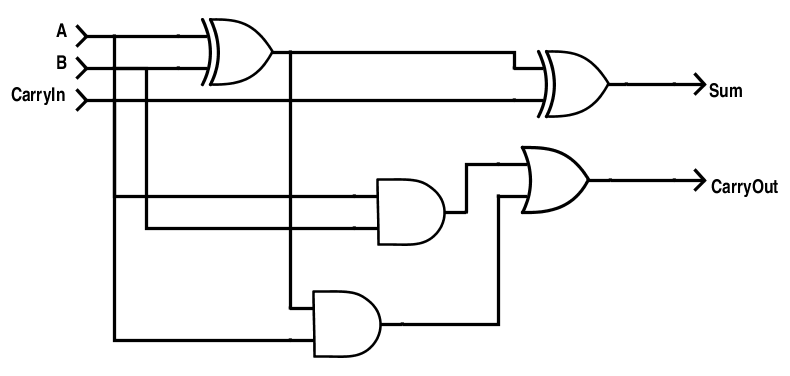
\includegraphics[width=0.75\textwidth]{adder.png}
				
	\caption{The circuit for a binary adder.}
\end{figure}

\subsection{The generated truth table}

Our circuit behaves as expected, following the previously defined rules.

\begin{lstlisting}
Cin A B | Sum Cout | Expected Output
0   0 0 | 0   0    | 0  1
0   1 0 | 1   0    | 1  0
0   0 1 | 1   0    | 1  0
0   1 1 | 0   1    | 0  1
1   0 0 | 1   0    | 1  0
1   1 0 | 0   1    | 0  1
1   0 1 | 0   1    | 0  1
1   1 1 | 1   1    | 1  1
\end{lstlisting}

\begin{figure}[H]
	\centering
	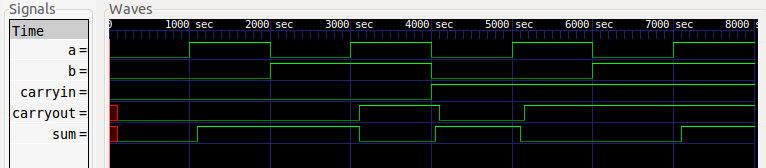
\includegraphics[width=0.75\textwidth]{../wave_forms/adder_wave.png}
				
	\caption{The waveform for a binary adder. Note the propagation delays due to the delays in the gates.}
\end{figure}

\section{The multiplexer}

The multiplexer takes in two bits: $A0$, $A1$. Using these two bits as a length-two binary number, the multiplexer selects one of its four outputs based on the inputs. It then sets this output to $1$, and all the others to $0$. and the carry-over from the previous addition.

The multiplexer is logically quite simple, but its circuit diagram is quite complex. To build this circuit, "and" each input with its corresponding index values from $A0$ and $A1$. Then, "or" all of these "anded" inputs together. All the wires not being indexed will be $0$, and the indexed input will be $1$ or $0$ depending on that input. The logic is illustrated in the source code in Appendix~\ref{plexer}.

\subsection{The generated truth table}

Our circuit behaves as expected. The only input that matters is the one that is indexed by $A0$ and $A1$.

\begin{lstlisting}
A0 A1| In0 In1 In2 In3 | Out | Expected Output
0  0 | 0   x   x   x   | 0   | 0
0  0 | 1   x   x   x   | 1   | 1
0  1 | x   0   x   x   | 0   | 0
0  1 | x   1   x   x   | 1   | 1
1  0 | x   x   0   x   | 0   | 0
1  0 | x   x   1   x   | 1   | 1
1  1 | x   x   x   0   | 0   | 0
1  1 | x   x   x   1   | 1   | 1
\end{lstlisting}

\begin{figure}[H]
	\centering
	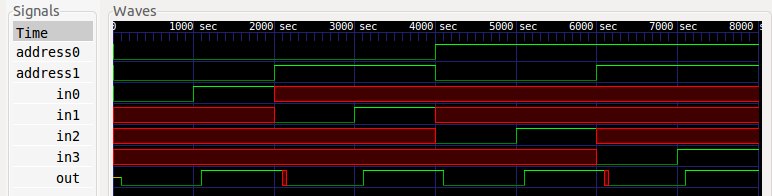
\includegraphics[width=0.75\textwidth]{../wave_forms/multiplexer_wave.png}
				
	\caption{The waveform for a mux.}
\end{figure}

\section{The decoder}

The decoder is similar to the mux. Instead of there being only one output wire, there are four. There are only three inputs. Two indices, and an $enable$ wire. The indexed output is set to the value of $enable$, and the rest to $0$. This is achieved by "and"ing together the index combinations with $enable$.

The logic is illustrated in the source code in Appendix~\ref{decoder}.

\subsection{The generated truth table}

Our circuit behaves as expected. The indexed output is set to $enable$.

\begin{lstlisting}
En A0 A1| O0 O1 O2 O3 | Expected Output
0  0  0 |  0  0  0  0 | All false
0  1  0 |  0  0  0  0 | All false
0  0  1 |  0  0  0  0 | All false
0  1  1 |  0  0  0  0 | All false
1  0  0 |  1  0  0  0 | O0 Only
1  1  0 |  0  1  0  0 | O1 Only
1  0  1 |  0  0  1  0 | O2 Only
1  1  1 |  0  0  0  1 | O3 Only
\end{lstlisting}

\begin{figure}[H]
	\centering
	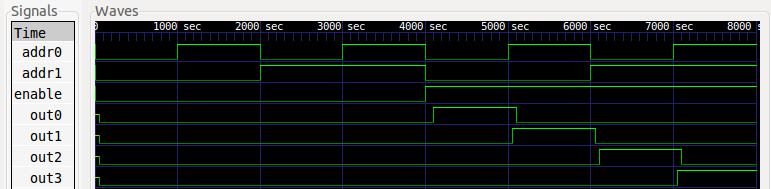
\includegraphics[width=0.75\textwidth]{../wave_forms/decoder_wave.png}
				
	\caption{The waveform for a decoder.}
\end{figure}

\appendix

\section{Adder code}

\lstinputlisting[language=Verilog]{../adder.v}

\section{Multiplexer code} \label{plexer}

\lstinputlisting[language=Verilog]{../multiplexer.v}

\section{Decoder code} \label{decoder}

\lstinputlisting[language=Verilog]{../decoder.v}

\end{document}
